\documentclass[14pt]{extbook}
\usepackage{multicol, enumerate, enumitem, hyperref, color, soul, setspace, parskip, fancyhdr} %General Packages
\usepackage{amssymb, amsthm, amsmath, latexsym, units, mathtools} %Math Packages
\everymath{\displaystyle} %All math in Display Style
% Packages with additional options
\usepackage[headsep=0.5cm,headheight=12pt, left=1 in,right= 1 in,top= 1 in,bottom= 1 in]{geometry}
\usepackage[usenames,dvipsnames]{xcolor}
\usepackage{dashrule}  % Package to use the command below to create lines between items
\newcommand{\litem}[1]{\item#1\hspace*{-1cm}\rule{\textwidth}{0.4pt}}
\pagestyle{fancy}
\lhead{Progress Quiz 1}
\chead{}
\rhead{Version B}
\lfoot{5899-4682}
\cfoot{}
\rfoot{Spring 2021}
\begin{document}

\begin{enumerate}
\litem{
Find the equation of the line described below. Write the linear equation as $ y=mx+b $ and choose the intervals that contain $m$ and $b$.\[ \text{Parallel to } 3 x - 7 y = 7 \text{ and passing through the point } (10, 8). \]\begin{enumerate}[label=\Alph*.]
\item \( m \in [1.99, 2.4] \hspace*{3mm} b \in [3.69, 4.22] \)
\item \( m \in [-0.05, 1.77] \hspace*{3mm} b \in [-4.68, -2.53] \)
\item \( m \in [-0.05, 1.77] \hspace*{3mm} b \in [-2.69, -1.22] \)
\item \( m \in [-0.44, 0.12] \hspace*{3mm} b \in [11.53, 13.45] \)
\item \( m \in [-0.05, 1.77] \hspace*{3mm} b \in [3.69, 4.22] \)

\end{enumerate} }
\litem{
Solve the linear equation below. Then, choose the interval that contains the solution.\[ \frac{-8x -4}{7} - \frac{7x + 5}{6} = \frac{-8x + 3}{4} \]\begin{enumerate}[label=\Alph*.]
\item \( x \in [-4.58, -0.58] \)
\item \( x \in [-7.96, -4.96] \)
\item \( x \in [-1.31, 2.69] \)
\item \( x \in [-41.77, -34.77] \)
\item \( \text{There are no real solutions.} \)

\end{enumerate} }
\litem{
Solve the equation below. Then, choose the interval that contains the solution.\[ -5(9x -12) = -15(-18x -14) \]\begin{enumerate}[label=\Alph*.]
\item \( x \in [0.79, 1.06] \)
\item \( x \in [-1.07, -0.77] \)
\item \( x \in [-0.64, -0.45] \)
\item \( x \in [-1.35, -1.19] \)
\item \( \text{There are no real solutions.} \)

\end{enumerate} }
\litem{
First, find the equation of the line containing the two points below. Then, write the equation as $ y=mx+b $ and choose the intervals that contain $m$ and $b$.\[ (-6, -7) \text{ and } (-2, 7) \]\begin{enumerate}[label=\Alph*.]
\item \( m \in [1.5, 7.5] \hspace*{3mm} b \in [13.72, 16.39] \)
\item \( m \in [1.5, 7.5] \hspace*{3mm} b \in [-14.47, -13.28] \)
\item \( m \in [-4.5, 0.5] \hspace*{3mm} b \in [-0.25, 0.59] \)
\item \( m \in [1.5, 7.5] \hspace*{3mm} b \in [-1.92, -0.84] \)
\item \( m \in [1.5, 7.5] \hspace*{3mm} b \in [8.3, 9.67] \)

\end{enumerate} }
\litem{
First, find the equation of the line containing the two points below. Then, write the equation as $ y=mx+b $ and choose the intervals that contain $m$ and $b$.\[ (-11, 3) \text{ and } (10, 7) \]\begin{enumerate}[label=\Alph*.]
\item \( m \in [-0.21, -0.15] \hspace*{3mm} b \in [8.4, 11.1] \)
\item \( m \in [0.05, 0.96] \hspace*{3mm} b \in [-5.6, -4] \)
\item \( m \in [0.05, 0.96] \hspace*{3mm} b \in [12.2, 17.1] \)
\item \( m \in [0.05, 0.96] \hspace*{3mm} b \in [-3.2, -2.4] \)
\item \( m \in [0.05, 0.96] \hspace*{3mm} b \in [1.2, 5.9] \)

\end{enumerate} }
\litem{
Write the equation of the line in the graph below in Standard form $Ax+By=C$. Then, choose the intervals that contain $A, B, \text{ and } C$.
\begin{center}
    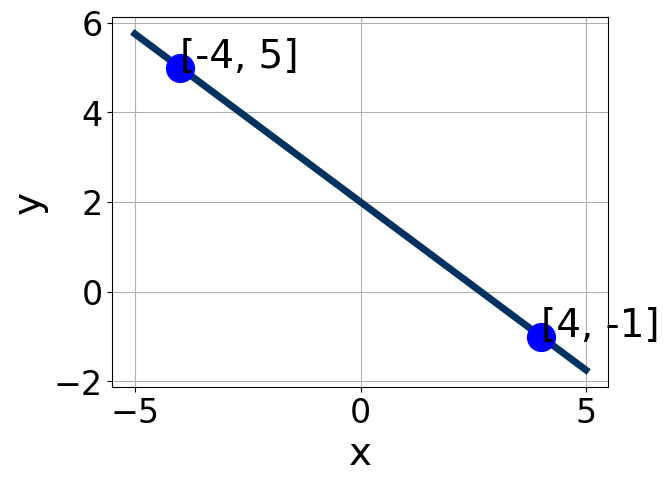
\includegraphics[width=0.5\textwidth]{../Figures/linearGraphToStandardCopyB.png}
\end{center}
\begin{enumerate}[label=\Alph*.]
\item \( A \in [-2.7, -1], \hspace{3mm} B \in [-1.2, -0.4], \text{ and } \hspace{3mm} C \in [1, 6] \)
\item \( A \in [-2.7, -1], \hspace{3mm} B \in [0.4, 2.3], \text{ and } \hspace{3mm} C \in [-8, -2] \)
\item \( A \in [3.8, 4.2], \hspace{3mm} B \in [-4.8, -1.3], \text{ and } \hspace{3mm} C \in [9, 12] \)
\item \( A \in [-4.2, -3.9], \hspace{3mm} B \in [1.6, 6.4], \text{ and } \hspace{3mm} C \in [-12, -7] \)
\item \( A \in [3.8, 4.2], \hspace{3mm} B \in [1.6, 6.4], \text{ and } \hspace{3mm} C \in [-12, -7] \)

\end{enumerate} }
\litem{
Write the equation of the line in the graph below in Standard form $Ax+By=C$. Then, choose the intervals that contain $A, B, \text{ and } C$.
\begin{center}
    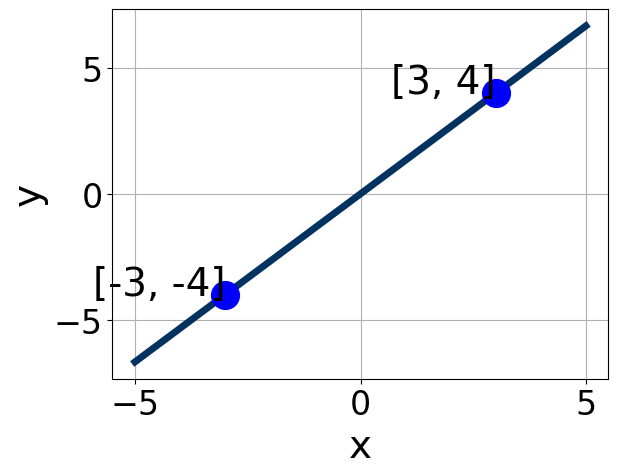
\includegraphics[width=0.5\textwidth]{../Figures/linearGraphToStandardB.png}
\end{center}
\begin{enumerate}[label=\Alph*.]
\item \( A \in [-0.85, 1.82], \hspace{3mm} B \in [-0.51, 1.37], \text{ and } \hspace{3mm} C \in [-4, 0] \)
\item \( A \in [-0.85, 1.82], \hspace{3mm} B \in [-2.01, -0.74], \text{ and } \hspace{3mm} C \in [4, 14] \)
\item \( A \in [-2.86, -1.21], \hspace{3mm} B \in [-6.01, -4.71], \text{ and } \hspace{3mm} C \in [15, 25] \)
\item \( A \in [0.78, 2.6], \hspace{3mm} B \in [4.78, 5.9], \text{ and } \hspace{3mm} C \in [-21, -9] \)
\item \( A \in [0.78, 2.6], \hspace{3mm} B \in [-6.01, -4.71], \text{ and } \hspace{3mm} C \in [15, 25] \)

\end{enumerate} }
\litem{
Solve the equation below. Then, choose the interval that contains the solution.\[ -12(18x + 16) = -4(-14x -7) \]\begin{enumerate}[label=\Alph*.]
\item \( x \in [-1.16, -0.83] \)
\item \( x \in [-0.68, -0.54] \)
\item \( x \in [-0.91, -0.63] \)
\item \( x \in [0.27, 0.62] \)
\item \( \text{There are no real solutions.} \)

\end{enumerate} }
\litem{
Find the equation of the line described below. Write the linear equation as $ y=mx+b $ and choose the intervals that contain $m$ and $b$.\[ \text{Perpendicular to } 8 x - 7 y = 4 \text{ and passing through the point } (-2, -9). \]\begin{enumerate}[label=\Alph*.]
\item \( m \in [-1.01, -0.67] \hspace*{3mm} b \in [-10.87, -10.74] \)
\item \( m \in [-1.01, -0.67] \hspace*{3mm} b \in [-7.17, -6.92] \)
\item \( m \in [-1.01, -0.67] \hspace*{3mm} b \in [10.72, 10.93] \)
\item \( m \in [-1.17, -1.11] \hspace*{3mm} b \in [-10.87, -10.74] \)
\item \( m \in [0.51, 1.28] \hspace*{3mm} b \in [-7.39, -7.18] \)

\end{enumerate} }
\litem{
Solve the linear equation below. Then, choose the interval that contains the solution.\[ \frac{7x + 8}{3} - \frac{6x + 5}{7} = \frac{3x -5}{5} \]\begin{enumerate}[label=\Alph*.]
\item \( x \in [-6, -3.8] \)
\item \( x \in [-4.4, -2.9] \)
\item \( x \in [1.2, 2.3] \)
\item \( x \in [-9.8, -7.1] \)
\item \( \text{There are no real solutions.} \)

\end{enumerate} }
\end{enumerate}

\end{document}